\subsection{Časovače a počítadlá}
\noindent

Ako názov napovedá, časovače sú určené na meranie času. Často ich nazývame aj počítadlá
pretože vo svojom základnom princípe časovače len počítajú počet dokončených periód zdrojových hodín.
Každý časovač má svoj vlastný register, kde je uložená jeho aktuálna hodnota a taktiež každý potrebuje zdroj hodín. V mikrokontroléroch často existuje niekoľko možných zdrojov
hodín a ich výber je možné určiť pomocou prepínača. Niektoré mikrokontroléry umožňujú aj použitie
externých hodín \cite{IntroductionMicrocontrollerTimers}. \par
Fungovanie časovača si najlepšie opíšeme na konkrétnom príklade.
Uvažujme časovač s 16-bitovým registrom a zdrojom hodín s frekvenciou 16 megahertzov. Po každom uplynutí cyklu v hodinách, časovač
zvýši hodnotu uloženú v registri o 1. Keďže časovač má k dispozícii 16-bitový register, maximálny počet možných hodnôt v registri je $2^{16}$ (65536, maximálna hodnota je 65365).
Po dosiahnutí maximálnej hodnoty register pretečie a časovač začne počítať znova od 0. Pri hodinách s frekvenciou 16 megahertzov časovač dosiahne maximálnu hodnotu registra približne každé 4 milisekundy. Vzorec pre výpočet spomínaného času je
$\frac{N-1}{Fr.}$, kde $N$ je počet hodnôt v registri a $Fr.$ je frekvencia hodín.
Pri pretečení registra natáva taktiež ešte jedna veľmi dôležitá udalosť. Časovač nastaví dopredu známy bit na logickú jednotku. Vďaka tomu dokážeme spúštať
kód v konkrétnom čase. To či bol daný bit nastavený je možné kontrolovať manuálne alebo na to zareagovať pomocou prerušenia, ktoré pri správnom nastavení vygeneruje procesor.
Tento proces sa opakuje stále dookola. Zmena hodnoty v
registri je zobrazená na obrázku č.\ref{figure:timer1}.

\begin{figure}[!h]
    \centering
    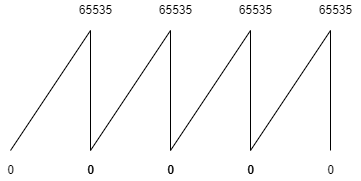
\includegraphics{img/timer.png}
    \caption{Zmena hodnoty v 16 bitovom registri časovača.}
    \label{figure:timer1}
\end{figure}

Popísaným spôbom môžeme dosiahnuť maximálne časové okno štyroch milisekúnd. Pri
bežnom používaní však často potrebujeme dosiahnuť dlhší interval, preto časovače
podporujú aj takzvané preddeličky (v anglickej literatúre sa používa pojem prescaler). Preddeličkou je možné znížiť frekvenciu počítadla a tým dosiahnúť dlhší interval medzi pretečením registra. Časovače majú pevne dané hodnoty preddeličiek a
najčastejšie ide o hodnoty 1 (nemá žiadny vpyv na frekvenciu), 8, 64, 256, 1024 atď. Pri použití preddeličky slúži na výpočet časového intervalu vzorec $\frac{N-1}{\frac{Fr.}{Pre.}}$ kde $N$ je počet hodnôt v registri, $Fr.$ je frekvencia hodín a $Pre.$ je honota preddeličky \cite{ElectronicBasics30}.

\subsubsection{Časovače a počítadlá v ARV mikrokontroléroch}
\noindent
Správanie a konfigurácia časovačov sa môže veľmi líšiť v závislosti od modelu procesora. V tejto diplomovej práci sa budeme venovať procesorom s architektúrov AVR, preto sa na časovače v tejto architektúre pozrieme konkrétnejšie.